% Options for packages loaded elsewhere
\PassOptionsToPackage{unicode}{hyperref}
\PassOptionsToPackage{hyphens}{url}
%
\documentclass[
  ignorenonframetext,
]{beamer}
\usepackage{pgfpages}
\setbeamertemplate{caption}[numbered]
\setbeamertemplate{caption label separator}{: }
\setbeamercolor{caption name}{fg=normal text.fg}
\beamertemplatenavigationsymbolsempty
% Prevent slide breaks in the middle of a paragraph
\widowpenalties 1 10000
\raggedbottom
\setbeamertemplate{part page}{
  \centering
  \begin{beamercolorbox}[sep=16pt,center]{part title}
    \usebeamerfont{part title}\insertpart\par
  \end{beamercolorbox}
}
\setbeamertemplate{section page}{
  \centering
  \begin{beamercolorbox}[sep=12pt,center]{part title}
    \usebeamerfont{section title}\insertsection\par
  \end{beamercolorbox}
}
\setbeamertemplate{subsection page}{
  \centering
  \begin{beamercolorbox}[sep=8pt,center]{part title}
    \usebeamerfont{subsection title}\insertsubsection\par
  \end{beamercolorbox}
}
\AtBeginPart{
  \frame{\partpage}
}
\AtBeginSection{
  \ifbibliography
  \else
    \frame{\sectionpage}
  \fi
}
\AtBeginSubsection{
  \frame{\subsectionpage}
}
\usepackage{amsmath,amssymb}
\usepackage{iftex}
\ifPDFTeX
  \usepackage[T1]{fontenc}
  \usepackage[utf8]{inputenc}
  \usepackage{textcomp} % provide euro and other symbols
\else % if luatex or xetex
  \usepackage{unicode-math} % this also loads fontspec
  \defaultfontfeatures{Scale=MatchLowercase}
  \defaultfontfeatures[\rmfamily]{Ligatures=TeX,Scale=1}
\fi
\usepackage{lmodern}
\ifPDFTeX\else
  % xetex/luatex font selection
\fi
% Use upquote if available, for straight quotes in verbatim environments
\IfFileExists{upquote.sty}{\usepackage{upquote}}{}
\IfFileExists{microtype.sty}{% use microtype if available
  \usepackage[]{microtype}
  \UseMicrotypeSet[protrusion]{basicmath} % disable protrusion for tt fonts
}{}
\makeatletter
\@ifundefined{KOMAClassName}{% if non-KOMA class
  \IfFileExists{parskip.sty}{%
    \usepackage{parskip}
  }{% else
    \setlength{\parindent}{0pt}
    \setlength{\parskip}{6pt plus 2pt minus 1pt}}
}{% if KOMA class
  \KOMAoptions{parskip=half}}
\makeatother
\usepackage{xcolor}
\newif\ifbibliography
\setlength{\emergencystretch}{3em} % prevent overfull lines
\providecommand{\tightlist}{%
  \setlength{\itemsep}{0pt}\setlength{\parskip}{0pt}}
\setcounter{secnumdepth}{-\maxdimen} % remove section numbering
\ifLuaTeX
  \usepackage{selnolig}  % disable illegal ligatures
\fi
\IfFileExists{bookmark.sty}{\usepackage{bookmark}}{\usepackage{hyperref}}
\IfFileExists{xurl.sty}{\usepackage{xurl}}{} % add URL line breaks if available
\urlstyle{same}
\hypersetup{
  pdftitle={TNC Integration and Subsidization as a Compliment to Public Transportation},
  pdfauthor={Charlie Berman},
  hidelinks,
  pdfcreator={LaTeX via pandoc}}

\title{TNC Integration and Subsidization as a Compliment to Public
Transportation}
\author{Charlie Berman}
\date{2024-03-12}

\begin{document}
\frame{\titlepage}

\begin{frame}{Background}
\protect\hypertarget{background}{}
\begin{itemize}
\tightlist
\item
  Declining Public Transportation Usage
\item
  Corresponds with the rise of Transportation Network Companies (TNCs)
\end{itemize}

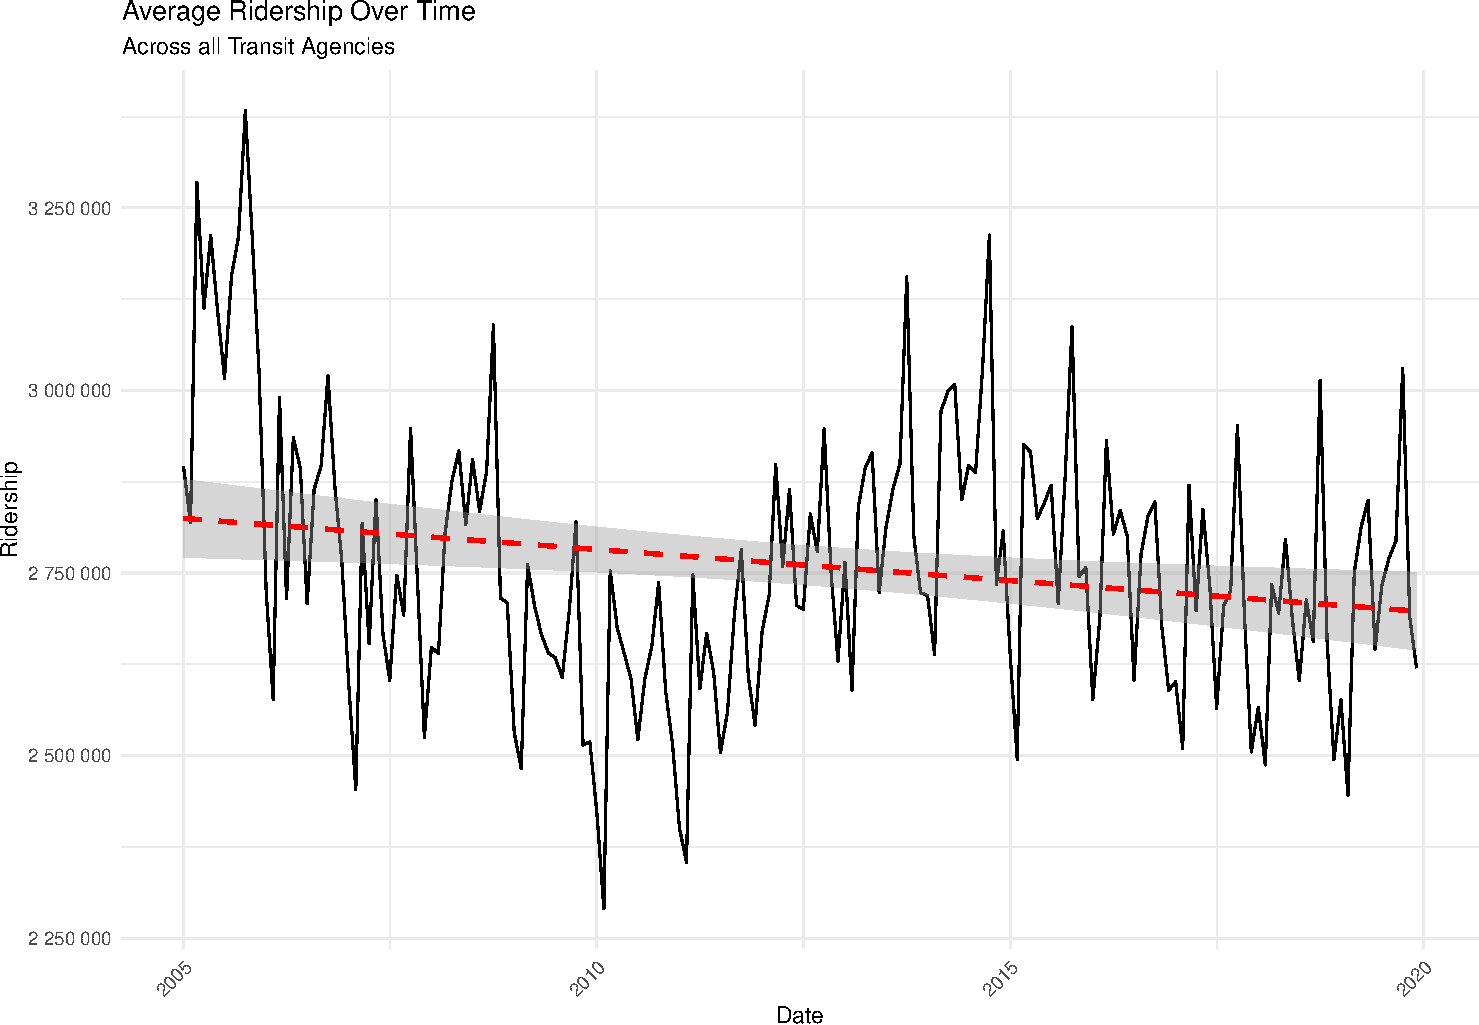
\includegraphics[width=0.7\linewidth]{detailed_proposal_files/figure-beamer/unnamed-chunk-1-1}
\end{frame}

\begin{frame}{Background}
\protect\hypertarget{background-1}{}
\begin{itemize}
\tightlist
\item
  Public transit companies partner with TNCs

  \begin{itemize}
  \tightlist
  \item
    Pinellas County subsidies
  \item
    Atlanta, GA MARTA on the Go
  \end{itemize}
\end{itemize}

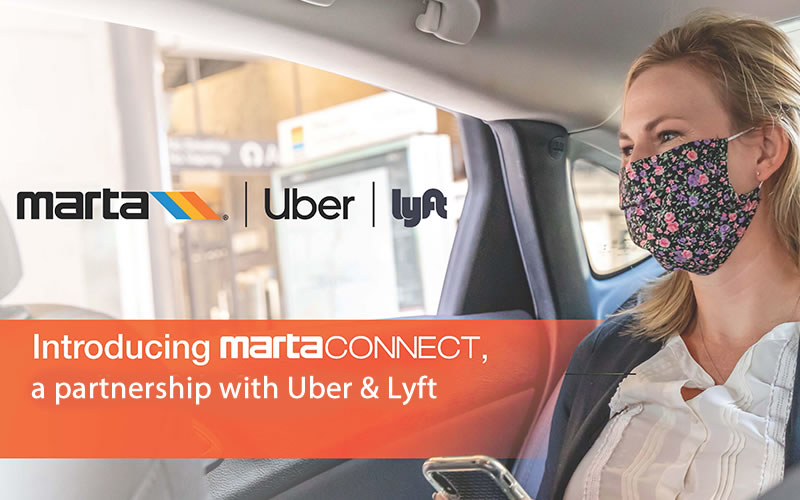
\includegraphics[width=0.7\linewidth]{martaconnect-page-banner2}
\end{frame}

\begin{frame}{Literature}
\protect\hypertarget{literature}{}
\begin{itemize}
\tightlist
\item
  Erhardt, et al.~(2022) claim TNCs are the biggest driver of transit
  ridership decline using NTD data
\item
  Hall, et al.~(2018) find that TNCs are a net compliment to public
  transit but lots of variation using diff-in-diff
\item
  Zhao (2019) finds that TNCs are a compliment to good transit,
  substitute to bad using monocentric city model
\item
  Agrawal, et al.~(2023) finds that subsidizing TNCs increases ridership
  substantially using monocentric city model
\end{itemize}
\end{frame}

\begin{frame}{Research Question}
\protect\hypertarget{research-question}{}
\begin{itemize}
\tightlist
\item
  What is the effect on ridership for public transportation agencies
  that partner with TNCs?

  \begin{itemize}
  \tightlist
  \item
    Subsidies
  \item
    Promotion(?)
  \end{itemize}
\end{itemize}
\end{frame}

\begin{frame}{Methodology}
\protect\hypertarget{methodology}{}
\begin{itemize}
\tightlist
\item
  Difference-in-difference

  \begin{itemize}
  \tightlist
  \item
    Treatment: Public transportation agencies that partner with TNCs
  \item
    Control: Public transportation agencies that do not partner with
    TNCs
  \item
    Time: Before and after partnership
  \end{itemize}
\item
  Considerations

  \begin{itemize}
  \tightlist
  \item
    Subsetting the dataset
  \item
    Partnership times. Will there be enough data post treatment?
  \end{itemize}
\end{itemize}
\end{frame}

\begin{frame}[fragile]{Data Sources}
\protect\hypertarget{data-sources}{}
\begin{itemize}
\tightlist
\item
  National Transit Database (NTD)

  \begin{itemize}
  \tightlist
  \item
    Contains monthly ridership data from 2005-2019 for all public
    transportation agencies that receive federal funding
  \end{itemize}
\item
  American Community Survey (ACS)

  \begin{itemize}
  \tightlist
  \item
    Contains yearly demographic data for all urbanized areas (+65,000
    population)
  \item
    Consider using CPS (monthly) \tiny
  \end{itemize}
\end{itemize}

\begin{verbatim}
## # A tibble: 6 x 26
##   agency    date       ridership ntd_id legacy_ntd_id status
##   <chr>     <date>         <dbl> <chr>  <chr>         <chr> 
## 1 2Plus Pa~ 2008-01-01      1144 10110  1110          Inact~
## 2 2Plus Pa~ 2008-02-01      1092 10110  1110          Inact~
## 3 2Plus Pa~ 2008-03-01      1050 10110  1110          Inact~
## 4 2Plus Pa~ 2008-04-01      1100 10110  1110          Inact~
## 5 2Plus Pa~ 2008-05-01      1056 10110  1110          Inact~
## 6 2Plus Pa~ 2008-06-01      1008 10110  1110          Inact~
## # i 20 more variables: reporter_type <chr>, uace_cd <chr>,
## #   uza_name <chr>, city <chr>, state <chr>, mode <chr>,
## #   tos <chr>, x3_mode <chr>, month <chr>, year <dbl>,
## #   geoid <chr>, med_age <dbl>, pop <dbl>, white <dbl>,
## #   black <dbl>, asian <dbl>, hispanic <dbl>,
## #   poverty <dbl>, med_house_income <dbl>, bach <dbl>
\end{verbatim}
\end{frame}

\begin{frame}[fragile]{Preliminary Results}
\protect\hypertarget{preliminary-results}{}
\begin{itemize}
\tightlist
\item
  Limited to FL
\item
  Diff-in-diff of Pinellas County vs.~rest of FL \tiny
\end{itemize}

\begin{verbatim}
##                                   didreg
## Dependent Var.:                ridership
##                                         
## Constant           2,235,049.5*** (29.2)
## pop                      0.372*** (17.9)
## white            -3,989,205.8*** (-50.7)
## med_house_income          26.0*** (22.2)
## poverty                 -1.97*** (-10.9)
## treated              414,098.4*** (19.0)
## time               -465,046.5*** (-24.8)
## treated x time        -37,688.4 (-0.787)
## Fixed-Effects:   -----------------------
## month                                 No
## ________________ _______________________
## VCOV type                            IID
## Observations                      13,732
## R2                                 0.361
## Within R2                             --
## 
##                                didreg_fe
## Dependent Var.:                ridership
##                                         
## Constant                                
## pop                      0.372*** (17.9)
## white            -3,989,679.6*** (-50.7)
## med_house_income          26.0*** (22.3)
## poverty                 -1.97*** (-10.9)
## treated              414,123.9*** (19.0)
## time               -465,860.5*** (-24.8)
## treated x time        -37,747.9 (-0.788)
## Fixed-Effects:   -----------------------
## month                                Yes
## ________________ _______________________
## VCOV type                            IID
## Observations                      13,732
## R2                                 0.362
## Within R2                          0.361
## ---
## Signif. codes: 0 '***' 0.001 '**' 0.01 '*' 0.05 '.' 0.1 ' ' 1
\end{verbatim}
\end{frame}

\begin{frame}{Potential Issues}
\protect\hypertarget{potential-issues}{}
\begin{itemize}
\tightlist
\item
  Classifying partnerships/finding information (changes over time)
\item
  Ensuring that all agencies are classified as treated or control
  correctly
\end{itemize}
\end{frame}

\begin{frame}{References}
\protect\hypertarget{references}{}
{[}Agrawal and Zhao, 2023{]} Agrawal, D. R. and Zhao, W. (2023). Taxing
uber. Journal of Public Economics, 221:104862.

{[}Erhardt et al., 2022{]} Erhardt, G. D., Hoque, J. M., Goyal, V.,
Berrebi, S., Brakewood, C., and Watkins, K. E. (2022). Why has public
transit ridership declined in the united states? Transportation Research
Part A: Policy and Practice, 161:68--87.

{[}Hall et al., 2018{]} Hall, J. D., Palsson, C., and Price, J. (2018).
Is uber a substitute or complement for public transit? Journal of Urban
Economics, 108:36--50.

{[}Zhao, 2019{]} Zhao, W. (2019). The long run effects of uber on public
transit, congestion, sprawl, and the environment.
\end{frame}

\end{document}
